\chapter{The HH$\rightarrow$4b analysis}

The search for the exact shape of the Higgs potential is an interesting endeavor as its not only  directly related to \ac{ewsb} but also could solve some fundamental questions about the nature of the universe as described in section \ref{sec:beyond_sm}. Since the Higgs interacts via Yukawa couplings from equation \ref{eq:yukawa_term} the coupling strengths for fermions are directly proportional to their mass and thus the Higgs couples most strongly to heavy particles. The main production modes at the \ac{lhc} are shown in figure \ref{fig:main_production_processes}. All couplings in the following are scaled with respect to their \ac{sm} values and are denoted with $\kappa_\mathrm{c} = c/c_\mathrm{sm}$ so that $\kappa_\mathrm{c}=1$ represents the \ac{sm} value of some coupling $c$.

The dominant Higgs pair production processes are shown in figure \ref{fig:main_production_processes}. The first \ac{ggf} two diagrams (a) and (b) have a cross-section of
$\sigma_\text{vbf HH}^\text{SM}=\qty[]{31.05}{fb}$ calculated at a center of mass energy of \qty[]{13}{TeV} at \ac{nnlo} \citep{Grazzini_2018} while the \ac{vbf} processes (c), (d) and (e) of figure \ref{fig:main_production_processes} have a production cross-section of
$\sigma_\text{vbf HH}^\text{SM}=\qty[]{1.73}{fb}$ at \ac{nnnlo} \citep{PhysRevD.98.114016}. A characteristic of the \ac{vbf} processes is that the Higgs pair products are accompanied by two additional quarks. The \ac{vbf} cross section is about \qty[]{3e4}{} times smaller than the production cross section for single Higgs $\sigma_\text{H}^\text{SM}=\qty[]{48.58}{pb}$ at the \ac{lhc} \citep{de2016arxiv} which already illustrates the challenge of discovering Higgs pairs in these final states.
\begin{figure}
    \centering
    \subfigure[]{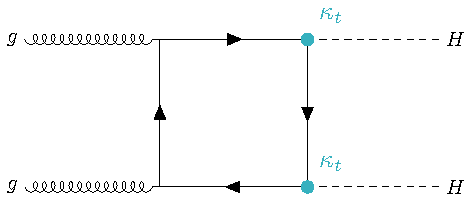
\includegraphics[width=.43\textwidth]{fig_01a}}\hspace{.06\textwidth}
    \subfigure[]{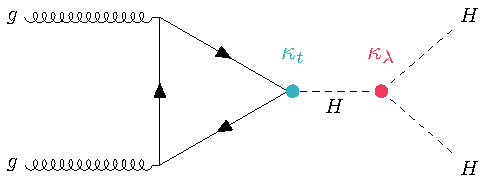
\includegraphics[width=.43\textwidth]{fig_01b}} \\
    \subfigure[]{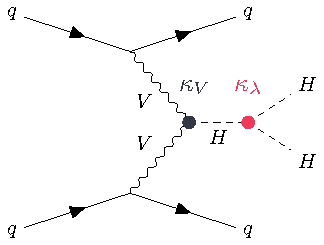
\includegraphics[width=.3\textwidth]{fig_02a}}\hspace{.01\textwidth}
    \subfigure[]{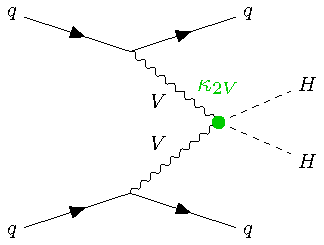
\includegraphics[width=.3\textwidth]{fig_02b}}\hspace{.01\textwidth}
    \subfigure[]{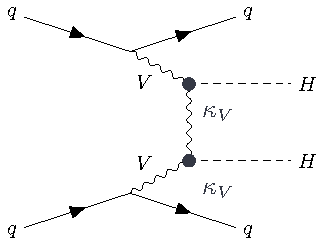
\includegraphics[width=.3\textwidth]{fig_02c}}
    \caption[]{Leading Higgs Pair production processes at the \ac{lhc}. (a), (b) shows \ac{ggf} and (c), (d), (e) \ac{vbf} processes. Adopted from \citep{aad2023search}.}
    \label{fig:main_production_processes}
\end{figure}
% higgs hat keine Ladung whatsoever cannot couple em or qcd 

\begin{figure}
    \centering
    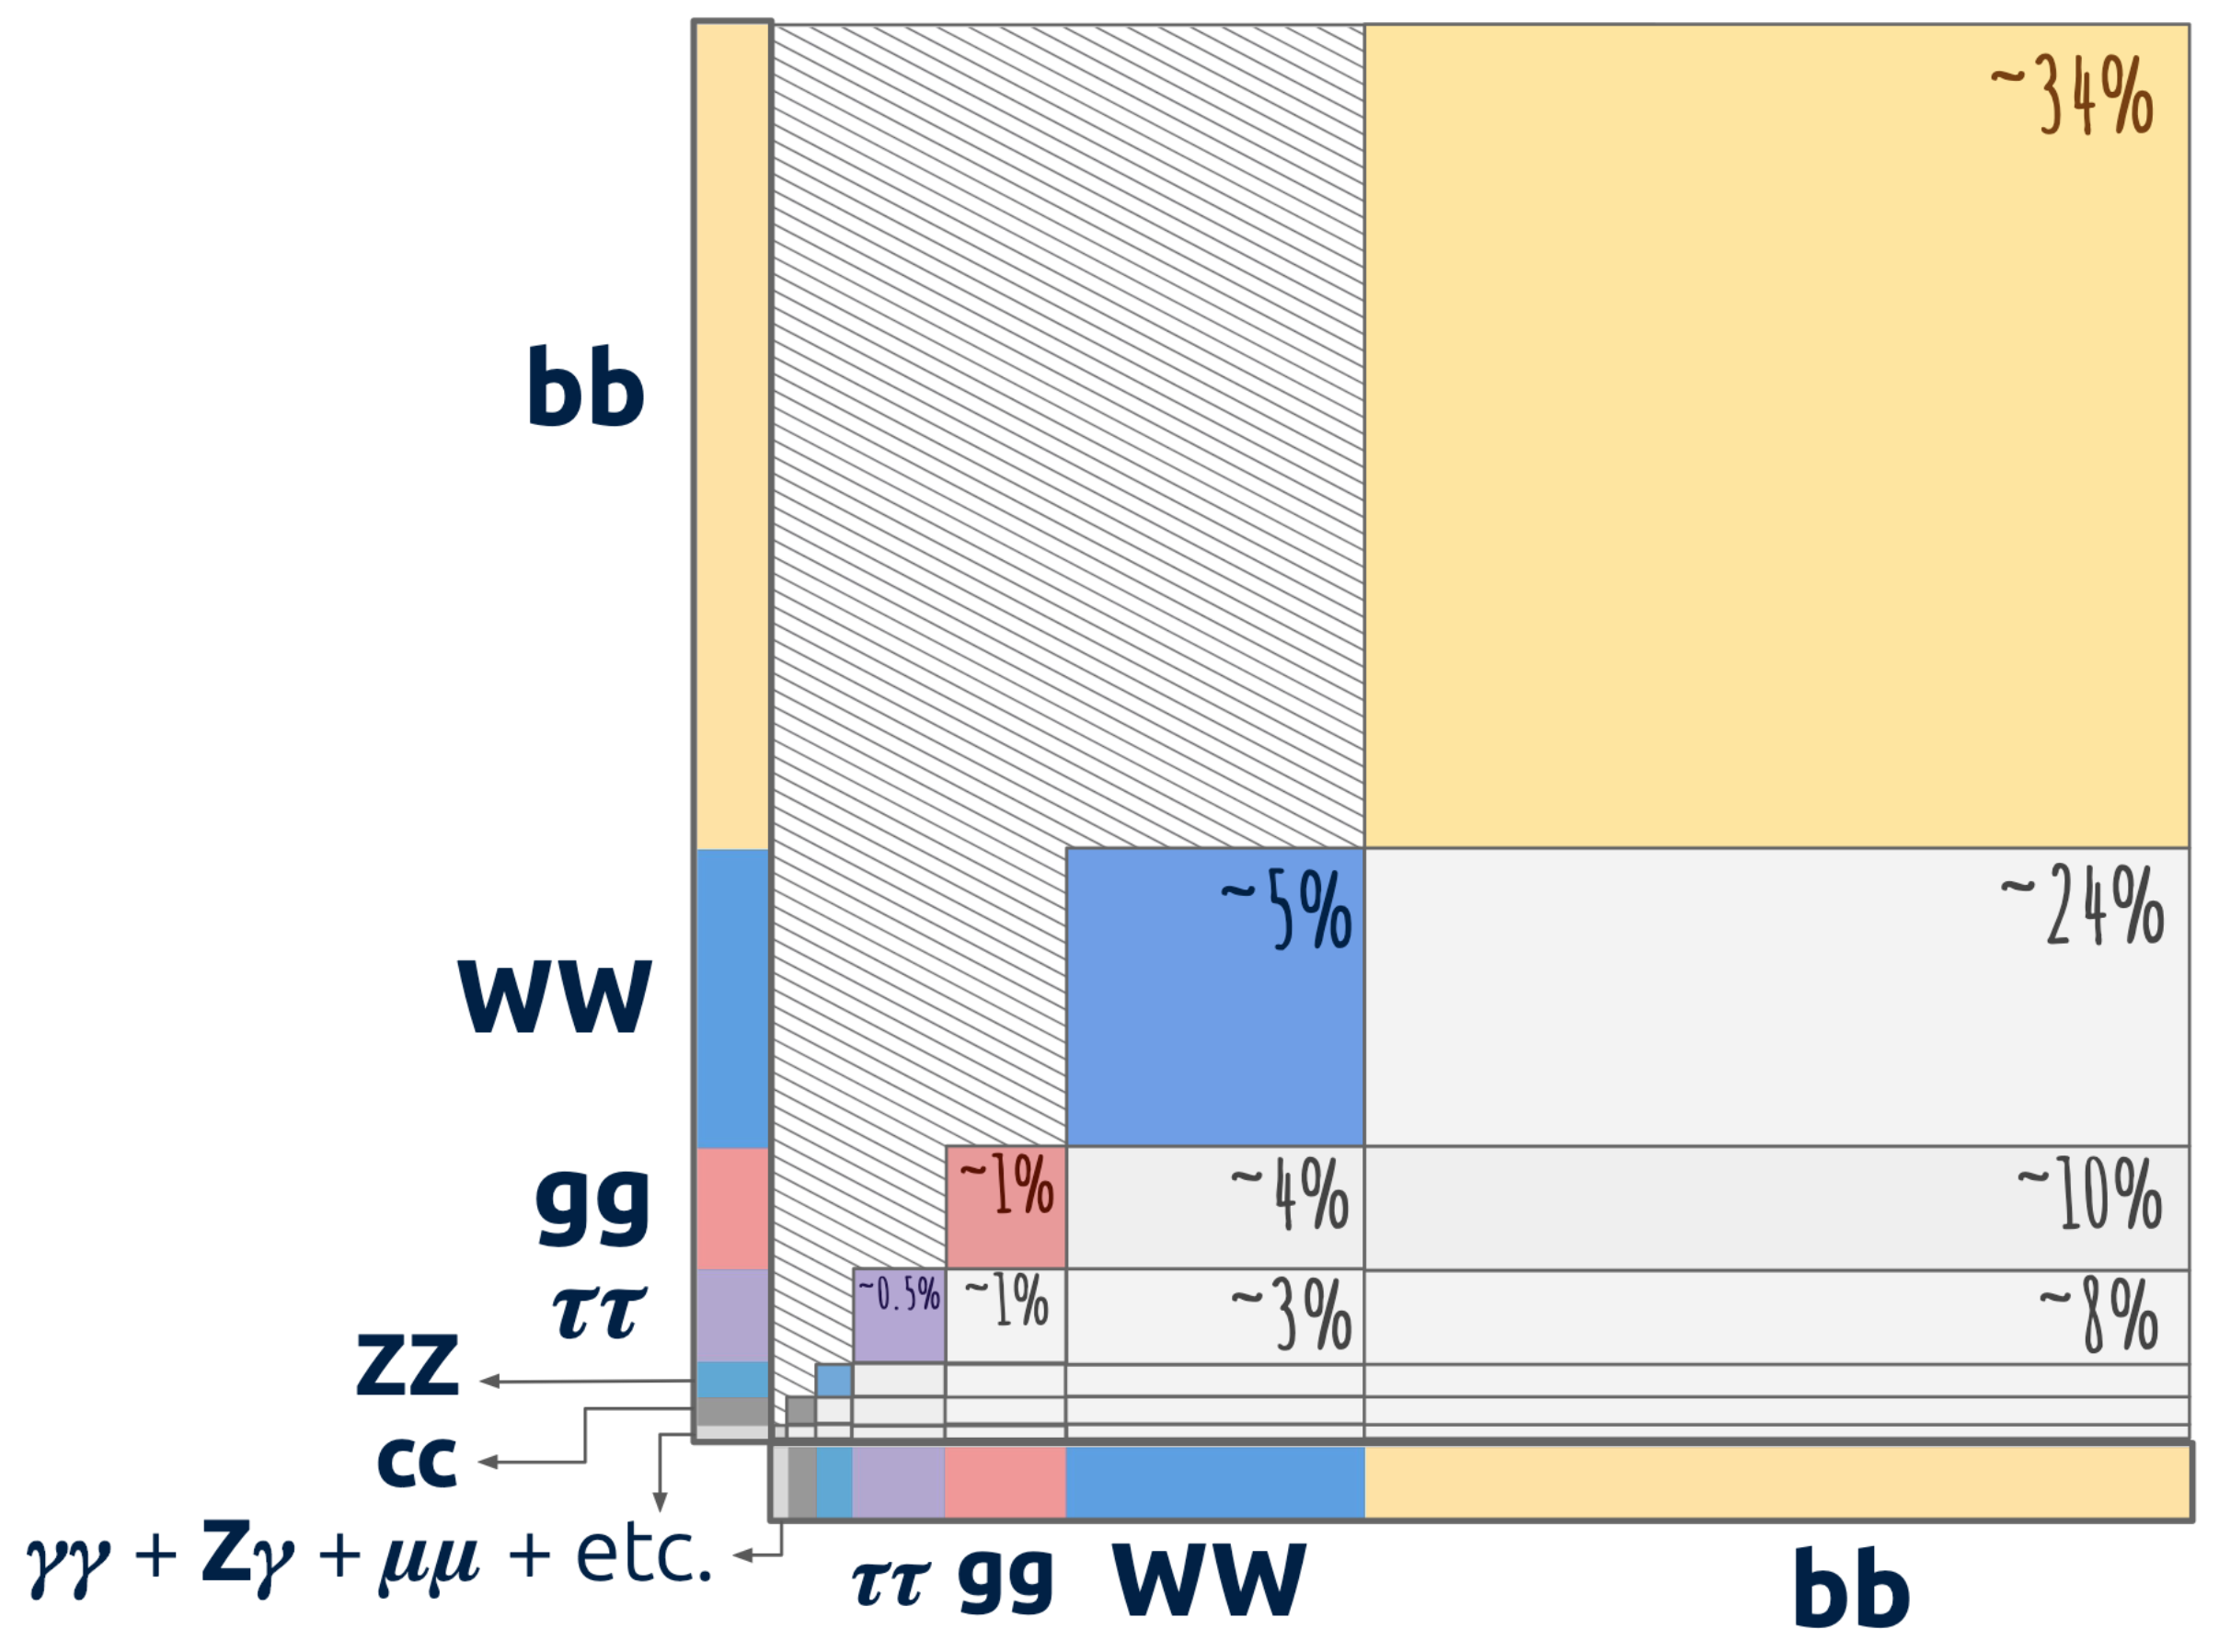
\includegraphics[width=0.7\textwidth]{branching_fraction_hh}
    \caption[]{Contributions of final states represented by area for a pair of Higgs \citep{Abbott:2708599}}
    \label{fig:branching_fraction_hh}
\end{figure}
Figure \ref{fig:branching_fraction_hh} reveals that an interesting channel is the final state with the largest branching fraction of about \qty[]{34}{percent} consisting of four $b$-quarks. However as this a fully hadronic final state it comes with the challenge of large \ac{qcd} backgrounds.

This work focuses on the boosted topology of highly energetic jets which do not allow reconstruction of $b$-jets individually but rather of final states consisting of two collimated $b$-jets inside a larger jet. The advantage of this selection is that it reduces greatly the \ac{qcd} backgrounds since highly energetic jets aare more likely to come from heavy particles such as $b$ quarks. Furthermore it is easy to trigger on events containing jets with large \pt. Although they represent a comparatively clean signal such events are rare and therefore have limited statistical power. For this reason other search strategies are better suited for the discovery of the Higgs pair production process.

A reason for the low cross-section is that diagrams (d) and (e) of figure \ref{fig:main_production_processes} cancel each other destructively for \ac{sm} values. In turn if $\ktwov$ is moved to non-\ac{sm} values the production cross-section increases significantly $\sigma_{\ktwov=0}\approx 20\sigma_{\ktwov=1}$ \citep{bishara2017higgs} and the decay products have much larger transverse momentum as shown in figure \ref{fig:kappa_2v_variations_mhh}.
\begin{figure}
    \centering
    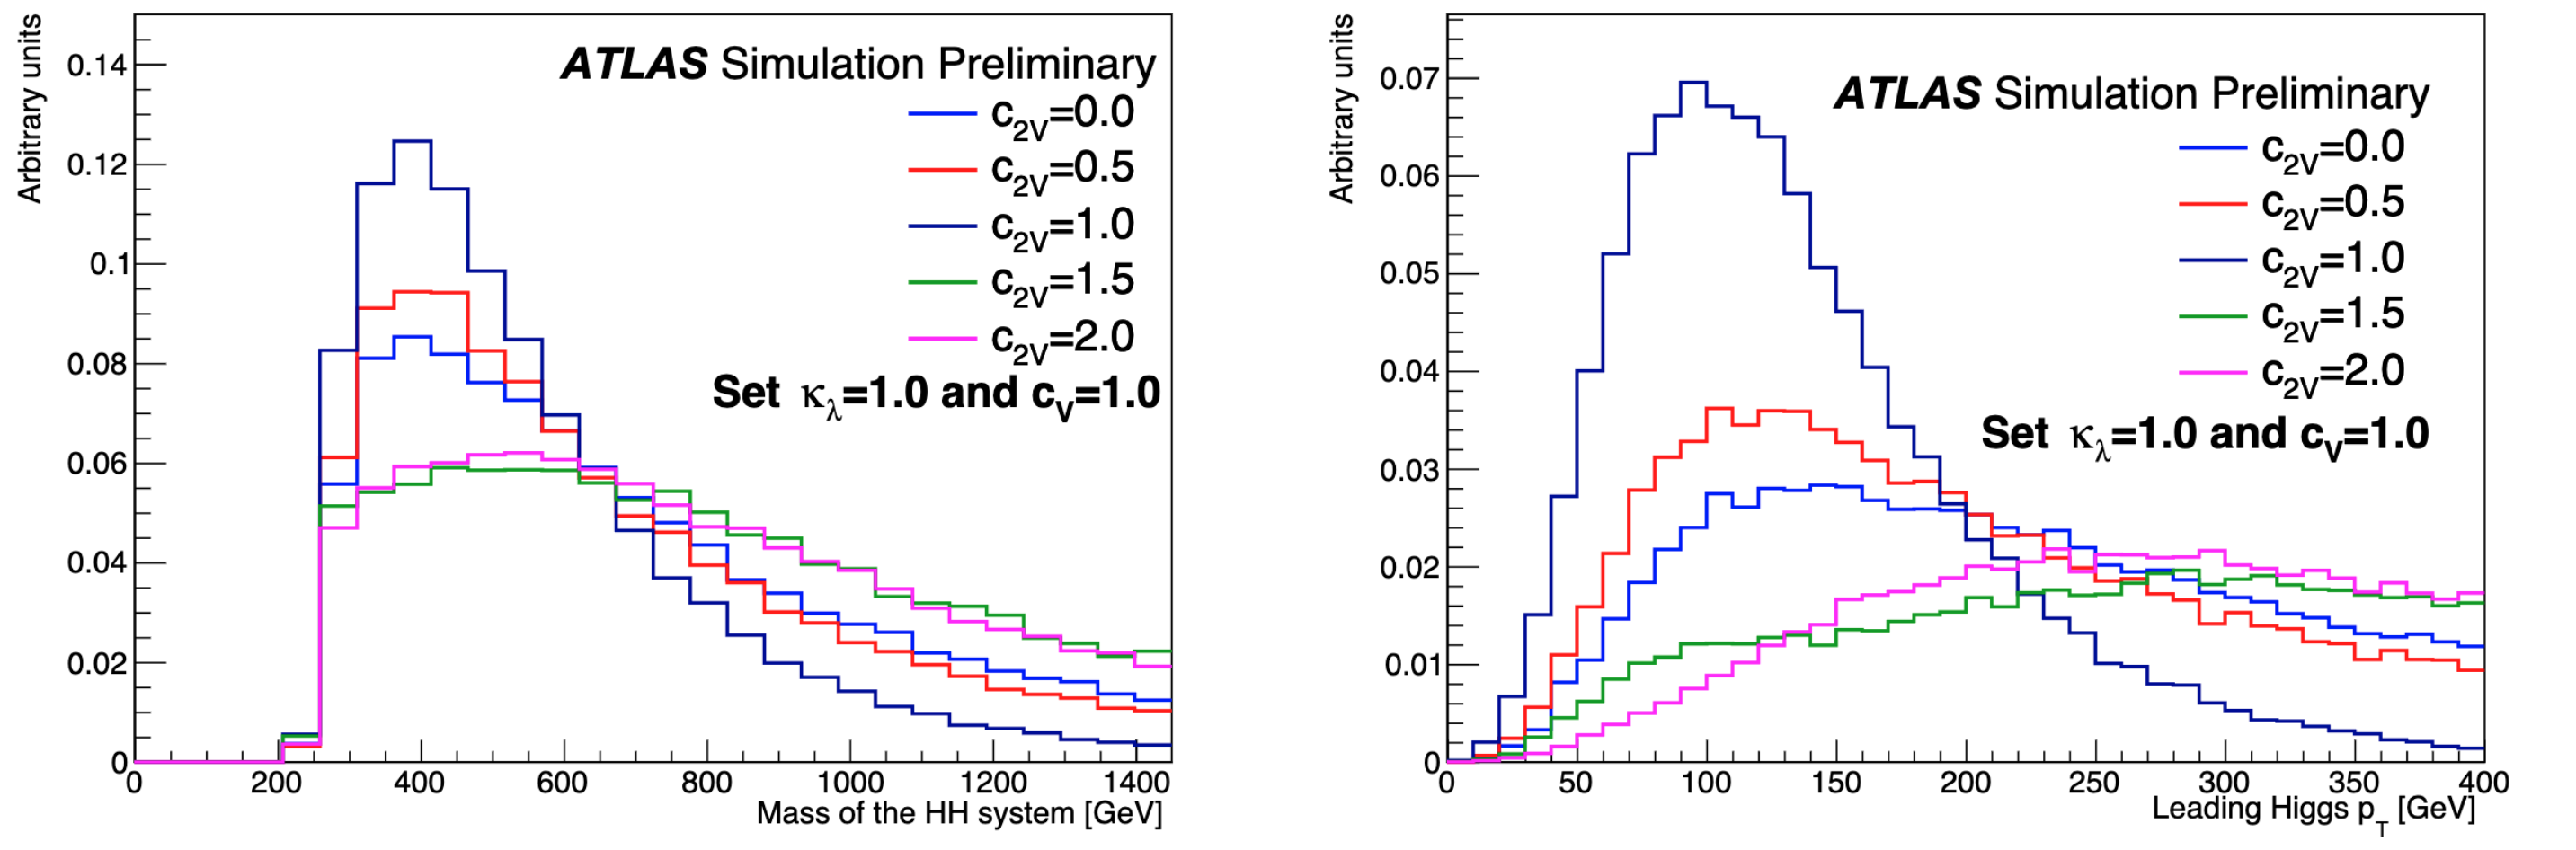
\includegraphics[width=1\textwidth]{kappa_2v_variations_mhh}
    \caption[]{Invariant mass of the Higgs pair system and the leading Higgs candidate jet \pt  reconstructed from simulation for different \ktwov. Adopted from \citep{ATL-PHYS-PUB-2019-007}.}
    \label{fig:kappa_2v_variations_mhh}
\end{figure}
Because of this behavior the power of this analysis lies in constraining and proving the existence of the \ktwov couplings within the \ac{sm} to which it is directly sensitive.



\section{Data and Monte Carlo Simulation}
This analysis uses the full run 2 data taken by \ac{atlas} between 2015 and 2018. The dataset contains \qty[]{140.1}{fb^{-1}} of data good for physics at a center of mass energy of \qty[]{13}{TeV} \citep{DAPR-2021-01}.

\ac{mc} generation in \ac{atlas} is done in three steps. At first at parton level events are generated with \textsc{MadGraph} (v.2.7.3p3.atlas6) \citep{alwall2014automated}. The output of this tool are stochastically sampled four vectors of the final states of the process of interest.

Afterwards \textsc{Pythia8} \citep{Sjostrand:2014zea} simulates the hadronization process. Because of the scaling behavior of \ac{qcd} described in \ref{sec:renormalization} partons inside a proton cannot be modeled since the perturbation ansatz of \ref{sec:qft} breaks down. However the partons momentum fraction can be deduced from \acp{pdf} by measuring them at some energy scale. For this the \textsc{NNPDF3.0nlo} \ac{pdf} is used by \textsc{Pythia8}. For normalization the \ac{sm} \ac{vbf} cross-section is multiplied by the 4b branching ratio $\mathcal{B}(4b)=0.3392$.


\red{add samples linear combination}
% https://www.overleaf.com/project/638e1930f926cd21d5264259
% linear combination
% Unfortunately, MC generation is computationally expensive and time-consuming. As such, only1443
% a handful of MC simulation samples for only a handful of coupling values are actually produced, and a1444
% sample combination technique is employed to model the signal hypothesis across the coupling parameter1445
% space
% https://trexfitter-docs.web.cern.ch/trexfitter-docs/model_building/expression/
% https://gitlab.cern.ch/hh4b/hh4b-boosted-vbf-limits/-/blob/main/create_workspaces/configs/k2V_parameterized_BDT_decorXbb.config?ref_type=heads#L285-331

\section{Analysis objects}
This section presents the details of the reconstruction for the objects used in the analysis. 
\subsection{Large Radius Jets}

\subsection{$X\rightarrow bb$ tagger}

% This work focuses on the boosted regime of the 4 $b$-quark final state. If jets are very boosted two $b$-jets can overlap and are reconstruct as variable radius jets inside a larger jet.
% as explained in section \ref{sec:vr_jets}.

% xbb tagger citation
% \citep{ATL-PHYS-PUB-2020-019}
% https://cds.cern.ch/record/2724739/files/ATL-PHYS-PUB-2020-019.pdf
% https://cds.cern.ch/record/2777811/files/ATL-PHYS-PUB-2021-035.pdf
% https://cds.cern.ch/record/2866601/files/ATL-PHYS-PUB-2023-021.pdf
% modeling

\subsection{Small Radius Jets}
\section{Analysis Strategy}
To fully capture the boosted topology of two jets that contain 2 collimated $b$-jets each so called Large R jets are used. These are formed with a radius parameter of $R=1.0$ for the Anti-$k_t$ clustering algorithm described in \ref{sec:anti_kt}.

region definitions
\subsection{Trigger}
\subsection{Event selection}
\subsubsection{Kinematic Selection}
\subsection{Background Estimation}

